\documentclass[12pt,letterpaper]{article}
\usepackage[utf8]{inputenc}
\usepackage[spanish,mexico]{babel}
\usepackage{amsmath}
\usepackage{amsfonts}
\usepackage{amssymb}
\usepackage{amsmath}
\usepackage[lmargin=3cm,rmargin=3cm,tmargin=3cm,bmargin=3cm]{geometry}

\usepackage{hyperref}
\usepackage{graphicx}
\usepackage{float}


\begin{document}

\title{Actividad 6: Período del Péndulo}
\author{Luisa Fernanda Orci Fernandez.}
\date{08 de Marzo del 2016}

\maketitle

\section*{Resumen de la actividad}

En esta actividad se llevó a cabo un análisis al cambiar de un péndulo simple a uno mas complejo, esto lo hicimos aumentando el tamaño de los periodos y de los ángulos, ya que entre mas grande sea el ángulo del péndulo mas complejo resulta su periodo. 

\section*{Péndulo}

\subsection*{Péndulo simple}

En otras actividades del presente curso ya hemos estudiado lo que es un péndulo simple y cuales son sus caracteristicas; que tiene una masa puntual, su movimiento describe un arco, hay falta de fricción, entre otras, pero este modelo solo funciona para ángulos pequeños. En estos casos resulta muy facil calcular el periodo con el uso de la siguiente ecuación:
$$ T = 2\pi\sqrt{\frac{l}{g}} $$ 
Esta se obtuvo a partir de la solución de la ecuación diferencial para un péndulo simple con condiciones iniciales ideales, también conocida como la Ley del periodo de Christiaan Huygens. Podemos observar que no se encuentra en terminos de su amplitud, ademas todo es constante a excepción de la longitud de la cuerda, esa si puede variar y de esa forma podríamos obtener distintos resultados para el periodo. 

\subsection*{Péndulo con ángulos mas grandes}
Para ángulos mayores a 30 grados, resulta mas complejo calcular el periodo, tan grande es el grado de complejidad que se necesita utilizar una herramienta computacional para integrar la ecuación que se obtiene a partir de la energía para la velocidad angular: $$ \frac{dt}{d\theta} = \sqrt{\frac{l}{2g}} \frac{1}{\sqrt{cos\theta - cos\theta_0}} $$ y esto se debe intregar sobre el el ciclo completo: $$ T = t(\theta_0 \rightarrow 0 \rightarrow -\theta_0 \rightarrow 0 \rightarrow \theta_0) $$ o también sobre dos veces medio ciclo: $$ T = 2t(\theta_0 \rightarrow 0 \rightarrow -\theta_0) $$ otra opción es integrando sobre cuatro veces un cuarto de ciclo:  $$ T = 4t(\theta_0 \rightarrow 0) $$ y esto nos lleva a la integral del péndulo para ángulos grandes: 

$$ T = 4\sqrt{\frac{l}{2g}} \int^{\theta_0}_0 \frac{1}{\sqrt{cos\theta - cos\theta_0}} $$

\section*{Actividad}

En esta actividad se nos pidió realizar una gráfica para de error relativo $\frac{T}{T_0}$ parecida a la figura n[umero 3 del artículo de Wikipedia $Pendulum$\cite{1},  anteriormente consultado. Esta gráfica la realizamos mediante la utilización de la función $scipy.integrate.quad$ de la biblioteca de $Scipy$. Se evaluó la integral anteriormente vista. También se nos solicitó ver como variaba el periodo en ángulos que van de cero a $\pi$.  El código obtenido fue el siguiente:

\begin{verbatim}
# PAQUETES
import numpy as gatito
from scipy import integrate
import matplotlib.pyplot as plt
import scipy as sp
import matplotlib as mpl
 

fig = plt.figure()
g = 9.8

# VECTORES
x = []
Ts = []
i = 0 # CONTADOR
 
while (i<=90):
        i=i+1 
        theta0 = (i*gatito.pi)/180 
        l = 1 
        f = lambda x: 1/gatito.sqrt(gatito.cos(x) - gatito.cos(theta0)) 
        
        #ESTUPIDA Y SENSUAL INTEGRAL
        
        F, erri = integrate.quad(f,0,theta0)
        T = 4 * gatito.sqrt(l/g) * (1/gatito.sqrt(2)) * F
       
        x.append(i)
        Ts.append(T)
T0 = 2*gatito.pi*gatito.sqrt(l/g)
T = Ts

#GRAFICA <3
plt.xlabel('Angulo') 
plt.ylabel('Error Relativo') 
plt.plot(Ts/T0) 
plt.show() 
\end{verbatim}
Y la gráfica obtenida fue la siguiente: 

\begin{center}

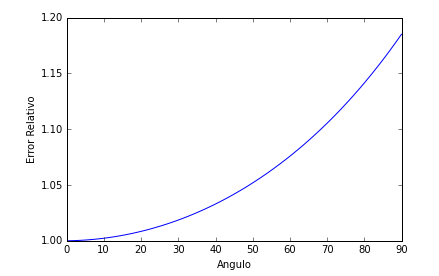
\includegraphics[scale=0.6]{ACTIVIDAD6.png}

\end{center}

\section*{Conclusiones}
Fue muy interesante el aprender esta manera mas rápida y eficiente de calcular integrales, y mas una de este tipo que se ve mucho en esta carrera, que es Licenciatura en Física.


\begin{thebibliography}{widestlabel}

\bibitem{1} Wikipedia, la enciclopedia libre \emph{Pendulum}, (2016, 08 de Marzo). Desde: \url{https://en.wikipedia.org/wiki/Pendulum_\%28mathematics\%29#Arbitrary-amplitude_period}

\end{thebibliography}

\end{document}